\chapter{Anwendungsfall}\label{chap:anwendungsfall}

Im folgenden Kapitel wird der Anwendungsfall vorgestellt, der als Grundlage zur Beantwortung der Fragestellungen dieser Arbeit (vgl. \autoref{sec:zielderArbeit}) dient. Der Anwendungsfall befasst sich mit der Untersuchung der Webanwendung Easy Web Leben \cite{easy_web}(\url{https://www.al-h.de/appserver/easyweb/}), im Folgenden Easy Web genannt. Die Plattform dient zur Kalkulation von Versicherungsprodukten im Bereich der Altersvorsorge. Im Folgenden werden zunächst einige relevante versicherungstechnische Terminologien eingeführt, anhand derer sich eine detaillierte Beschreibung der Easy Web-Plattform anschließt. Daraufhin wird die konkrete Methodik und Implementierung zur Beantwortung der Fragestellungen erläutert, zudem die Ergebnisse der korrespondierenden Untersuchungen vorgestellt.

\section{Vorstellung des Testobjekts}\label{sec:testobjekt}

Das 'Beratungscockpit' Easy Web \cite{easy_web} soll Vermittelnde und Kund*innen der ALH-Gruppe bei der Ermittlung der individuellen Bedürfnisse im Bereich der privaten und betrieblichen Altersvorsorge unterstützen. Dafür steht eine Reihe verschiedener Produkte und Tarife zur Verfügung, die anhand unterschiedlicher Parameter an die individuellen Anforderungen der Kund*innen angepasst werden können und letztlich in einem konkreten Antrag zum Abschluss einer Versicherung münden können. Easy Web ermittelt parallel dazu anhand der eingegebenen Parameter die zugehörige Rentenleistung.

Easy Web unterscheidet grundlegend zwischen Tarifen der privaten Vorsorge und der betrieblichen Altersvorsorge (bAV). Der Anwendungsfall dieser Arbeit fokussiert sich auf den Bereich der bAV, die Erkenntnisse lassen sich jedoch auch auf den Bereich der privaten Altersvorsorge übertragen.

\subsection{Versicherungstechnische Grundlagen}\label{subsec:versicherungsgrundlagen}

Die betriebliche Altersvorsorge (bAV) hat im deutschen Rentensystem gemeinsam mit der gesetzlichen und der privaten Vorsorge das Ziel, zu 'einer angemessenen Gesamtversorgung beim Ausscheiden aus dem Arbeitsleben' \cite[S. 12]{buttler2017einfuehrung} jeder Person beizutragen. Die gesetzliche, private und betriebliche Altersvorsorge werden in diesem Zusammenhang auch häufig als die drei Säulen des deutschen Rentensystems bezeichnet \cite[S. 3]{plato2016betriebliche}. 

Der Begriff der bAV bezeichnet beinhaltet 'alle Leistungen, die einem Arbeitnehmer zur Altersvorsorge, Hinterbliebenenversorgung oder Invaliditätsversorgung von seinem Arbeitgeber aus Anlass des Arbeitsverhältnisses zugesagt worden sind' \cite[S. 1]{buttler2017einfuehrung}. Dies bedeutet, dass im Wesentlichen Vorsorgeleistungen der klassischen Rentenversicherungen durch eine bAV ermöglicht werden können, aber auch Erwerbsminderungsrenten, Berufsunfähigkeitsrenten oder Risiko-Lebensversicherungen. 

Ursprünglich wurde die bAV als 'zusätzliche Sozialleistung des Arbeitgebers' \cite[S. 7]{buttler2017einfuehrung} eingeführt, sodass die Finanzierung der bAV aus wirtschaftlicher Sicht einzig und allein über separate Beiträge des Arbeitgebers erfolgte (Arbeitgeber-finanziert). Seit dem Jahr 2002 besitzt jeder Arbeitnehmer das Recht auf Umwandlung seines Lohnes für die Nutzung einer bAV \cite[S. 23]{buttler2017einfuehrung}, zudem muss dieses Vorhaben vom Arbeitgeber nach §1 a BetrAVG mit einem Zuschuss unterstützt werden \cite[S. 29]{buttler2017einfuehrung}, falls dieser Sozialversicherungsbeiträge durch die Entgeldumwandlung einspart. Dementsprechend kann die Finanzierung der bAV inzwischen auch durch den Arbeitnehmer erfolgen (Arbeitnehmer-finanziert) oder als Mischform bei der sowohl Arbeitgeber als auch Arbeitnehmer Beiträge leisten (Misch-finanziert).

Für die konkrete Ausgestaltung einer bAV stehen verschiedene Durchführungswege zur Verfügung, die im Folgenden basierend auf Buttler und Keller \cite{buttler2017einfuehrung} vorgestellt werden:

\paragraph*{Direktzusage}
Bei der Direktzusage übernimmt der Arbeitgeber die unmittelbare Verantwortung für die mit dem Arbeitnehmer getroffenen Vereinbarungen über die Erbringung einer Vorsorgeleistung. Der Arbeitnehmer besitzt einen Rechtsanspruch auf die versprochene Leistung gegenüber dem Arbeitgeber. Diesen weist der Arbeitgeber in seiner Bilanz als Pensionsrückstellungen aus. Zusätzlich kann der Arbeitgeber die versprochenen Leistungen über eine Rückdeckungsversicherung absichern. Finanziert wird die Direktzusage üblicherweise durch den Arbeitgeber  (Arbeitgeber-finanziert), eine Entgeldwandlung ist jedoch auch möglich (Arbeitnehmer-finanziert) \cite[S. 140]{buttler2017einfuehrung}.

\paragraph*{Direktversicherung}

Die Direktversicherung beschreibt das Vorgehen, bei welchem der Arbeitgeber eine Lebensversicherung auf das Leben des Arbeitnehmers bei einer Lebensversicherungsgesellschaft abschließt und die Beiträge übermittelt. Versicherungsnehmer ist somit der Arbeitgeber, bezugsberechtigt für die abgeschlossene Versicherungsleistung sind jedoch der Arbeitnehmer beziehungsweise dessen Hinterbliebene. Getragen wird die Direktversicherung allein vom Arbeitnehmer als Abzug vom Bruttolohn (Arbeitnehmer-finanziert), allein vom Arbeitgeber als separate Arbeitgeberleistung (Arbeitgeber-finanziert) oder als Mischform (Misch-finanziert) beider zuvor aufgeführten Varianten \cite[S. 33]{plato2016betriebliche}.

\paragraph*{Unterstützungskasse}
Die Unterstützungskasse ist eine von einem oder mehreren Trägerunternehmen etablierte Versorgungseinrichtung, die rechtlich selbstständig arbeitet und die Vorsorgeleistungen der bAV für die Arbeitnehmer der beteiligten Unternehmen übernimmt. Die Unterstützungskasse fungiert dabei nur als Dienstleister für die betroffenen Unternehmen, rechtlich verbleibt der Anspruch der Versicherungsleistung des Arbeitnehmers beim Arbeitgeber. Unterstützungskassen werden entweder durch die Beiträge zur Entgeldumwandlung der Arbeitnehmer (Arbeitnehmer-finanziert) oder über direkte Zuwendungen der Arbeitgeber (Arbeitgeber-finanziert) finanziert. %Sie agieren darüber hinaus frei in Bezug auf die Anlage ihrer Kapitalmittel, sodass sie über Kapitalanlagen Einkommensquellen erschließen können. Sie werden in rückgedeckte und paschaldotierte Unterstützungskassen unterschieden: Rückgedeckte Unterstützungskassen legen ihr Vermögen vollständig in Rückdeckungsversicherungen an, sodass die vereinbarte Versicherungsleistung mit dem Arbeitnehmer exakt abgesichert ist. Pauschaldotierte Unterstützungskasse agieren flexibler in ihrer Anlage, häufig in Form einer 'vollständigen Vermögensanlage per Darlehensgewährung ans Trägerunternehmen' \cite[S. 11]{buttler2017einfuehrung}.

\paragraph*{Pensionskasse}

Pensionskassen sind Versicherungsunternehmen, die sich im Gegensatz zu Lebensversicherungsunternehmen ausschließlich um die Durchführung von Rentenversicherungen im Rahmen von bAV-Verträgen kümmern. Konzeptionell gleicht die Durchführung einer bAV via Pensionskasse in weiten Teilen der Direktversicherung, Beiträge werden wie bei der Direktversicherung vom Arbeitgeber übermittelt. Die Finanzierung erfolgt wie bei der Direktversicherung über den Arbeitnehmer (Arbeitnehmer-finanziert) oder Arbeitgeber (Arbeitgeber-finanziert) allein oder gemeinsam (Misch-finanziert). 

Bis 2005 wurden Pensionskassen im Vergleich zu allgemeinen Lebensversicherern steuerlich besser gestellt, aktuell unterscheiden sich die beiden Durchführungswege nur marginal: So erhalten Arbeitnehmer ihre Versicherungsleistung im Falle der Pensionskasse erst bei Beendigung ihrer Erwerbstätigkeit und nicht zu einem vordefinierten Zeitpunkt wie bei einer Direktversicherung \cite[S. 191]{buttler2017einfuehrung}. Zudem entfallen bei der Pensionskasse bei einem Unternehmensaustritt mit einem Pensionskassenvertrag steuerliche Vorteile für den Arbeitnehmer, falls dieser weiterhin privat Beiträge entrichtet \cite[S. 192]{buttler2017einfuehrung}.

\paragraph*{Pensionsfonds}

Der Pensionsfonds existiert seit 2002 als zusätzlicher Durchführungsweg der bAV. Wie bei der Direktversicherung und der Pensionskasse auch agiert ein Pensionsfonds als rechtlich selbständiger Versorgungsträger, der Arbeitnehmern bei Abschluss eines bAV-Vertrags über den Arbeitgeber einen Rechtsanspruch auf Versicherungsleistungen einräumt. Die bAV-Durchführung via Pensionsfonds ermöglicht im Vergleich zur Direktversicherung und Pensionskasse größere Freiheiten in Bezug auf den Kalkulationszins, dieser wird im Falle des Pensionsfonds jedoch nicht gegenüber dem leistungsberechtigten Arbeitnehmer garantiert. Falls der Pensionsfonds diesen Zins auf dem Kapitalmarkt nicht erwirtschaften kann, muss somit der Arbeitnehmer mit einer geringeren Leistung auskommen oder der Arbeitgeber die Versorgungslücke nachfinanzieren. 


\begin{comment}
\hspace{1cm}Tabelle \ref{tab:finanzierungDurchfuehrungswege} fasst die Finanzierungsarten und Durchführungswege der bAV zusammen:

\begin{table}[h!]
\footnotesize
\begin{tabularx}{\textwidth}{|l|Y|Y|Y|l|}
\hline
\cellcolor{grauinfo}Durchführungsweg    & \cellcolor{grauinfo}Arbeitgeber-finanziert & \cellcolor{grauinfo}Arbeitnehmer-finanziert & \cellcolor{grauinfo}Misch-finanziert & \cellcolor{grauinfo}Bemerkung                  \\ \hline
Direktzusage        & \cmark                 & \cmark                  & \xmark           &                            \\ \hline
Direktversicherung  & \cmark                 & \cmark                  & \cmark           & Unterliegt § 3 Nr. 62 EStG \\ \hline
Unterstützungskasse & \cmark                 & \cmark                  & \xmark           &                            \\ \hline
Pensionskasse       & \cmark                 & \cmark                  & \cmark           & Unterliegt § 3 Nr. 62 EStG \\ \hline
Pensionsfonds       & \cmark                 & \cmark                  & \cmark           & Unterliegt § 3 Nr. 62 EStG \\ \hline
\end{tabularx}
\normalsize
\caption{Übersicht über die Durchführungswege und Finanzierungsarten der betrieblichen Altersvorsorge}.
\label{tab:finanzierungDurchfuehrungswege}
\end{table}

\end{comment}

\hspace{1cm}Für die Durchführungswege Direktversicherung, Pensionskasse und Pensionsfonds gilt, dass der Gesetzgeber die Beiträge zur bAV bis zu einer vordefinierten Grenze steuerfrei stellt und somit die Brutto-Steuerlast des Arbeitnehmers reduziert wird \cite[S. 109]{buttler2017einfuehrung}. Im Leistungsfall müssen die ausbezahlten Rentenbeiträge jedoch regulär versteuert werden \cite[S. 122]{buttler2017einfuehrung}. Dabei profitieren Arbeitnehmer meist von einem niedrigeren Steuersatz im Rentenalter als zur Zeit der Berufstätigkeit \cite{verbraucherzentrale}. 

§ 3 Nr. 63 EStG regelt die Grenzen für die Beitragsfreistellungen: Bis zum Jahr 2017 war die Steuerfreiheit bei den aufgeführten Durchführungswegen auf 4\% der Beitragsbemessungsgrenze der gesetzlichen Rentenversicherung (West) fixiert -- plus weitere 1.800 Euro, falls kein weiterer bAV-Vertrag unter Nutzung der Pauschalbesteuerung durch § 40 b EStG bestand \cite[S. 111]{buttler2017einfuehrung}. 

§ 40 b EStG ermöglichte bis 2004 die Beiträge zur bAV mit einer pauschalen Steuer von 20\% zu versteuern \cite[S. 113]{buttler2017einfuehrung}. Seitdem besteht die Möglichkeit zur Pauschalbesteuerung nur noch unter bestimmten Voraussetzungen wie bei Verträgen von umlagefinanzierten Pensionskassen oder bei bestehenden Altverträgen \cite[S. 113]{buttler2017einfuehrung}. Unter anderem erfordert die Anwendung von § 40 b EStG auch, dass der Arbeitnehmer beim Abschluss des bAV-Vertrages in seinem ersten Arbeitsverhältnis war \cite[S. 116]{buttler2017einfuehrung}. Der Gesetzgeber begrenzt die Nutzung der Steuerpauschalisierung nach § 40 b EStG auf 1.752 Euro je Arbeitnehmer \cite[S. 116]{buttler2017einfuehrung}. Falls der Vertrag im Rahmen eines Gruppenvertrages mehrerer Arbeitnehmer abgeschlossen wurde und der jährliche Aufwand des Arbeitgebers pro Arbeitnehmer im Durchschnitt nicht 1.752 Euro überschreitet, erhöht sich dieser Maximalbetrag auf 2.148 Euro \cite[S. 117]{buttler2017einfuehrung}.

Seit dem 01.01.2018 entfällt die damalige in § 3 Nr. 63 EStG festgeschriebene zusätzliche Förderung von 1.800 Euro, falls die Pauschalbesteuerung durch § 40 b EStG nicht genutzt wird \cite[S. 111]{buttler2017einfuehrung}. Die Fördergrenze für die Direktversicherung, Pensionskasse und Pensionsfonds beträgt nun einheitlich 8\% der Beitragsbemessungsgrenze der gesetzlichen Rentenversicherung (West) \cite[S. 111]{buttler2017einfuehrung}). Hat ein Arbeitnehmer jedoch vor dem 01.01.2018 einen Beitrag nach § 40 b Absatz 1 und 2 EStG a.F. pauschal besteuern lassen, kann dieser auch weiterhin durch die Pauschalbesteurung von § 40 b EStG erfasst werden \cite[S. 114 f.]{buttler2017einfuehrung}: Dieser Beitrag wird dann von der erhöhten 8\%-Fördergrenze abgezogen, damit Arbeitnehmer nicht zu sehr ihren steuerlichen Förderbeitrag ausweiten können \cite[S. 111]{buttler2017einfuehrung}. 

Im Jahr 2021 lag die die Beitragsbemessungsgrenze der gesetzlichen Rentenversicherung für Westdeutschland bei 85.200 Euro jährlich \cite{bbg2021}, was somit einer Fördergrenze von 6.816 Euro im Sinne des § 3 Nr. 62 EStG entspricht.

Bei den Durchführungswegen der Direktzusage und Unterstützungskasse verbleibt der Leistungsanspruch des Arbeitnehmers beim Arbeitgeber und wird nicht auf ein drittes Unternehmen übertragen. Der Arbeitnehmer ist nicht 'verfügungsberechtigt' \cite[S. 137]{buttler2017einfuehrung} über die Mittel, die der Arbeitgeber zurückstellt, weshalb die Beiträge in diesen Fällen grundsätzlich nicht zu versteuern sind \cite[S. 138]{buttler2017einfuehrung}. Erst bei Eintritt des Versorgungsfalles erhält der Arbeitnehmer Zugriff auf die Leistungen, sodass diese Einkünfte dann im Rahmen von 'Einkünften nichtselbständiger Arbeit' \cite[S. 138]{buttler2017einfuehrung} versteuert werden müssen. Es existiert jedoch ein Versorgungsfreibetrag (§ 19 Abs. 2 EStG), der die Höhe der Besteuerung abmildert \cite[S. 138]{buttler2017einfuehrung}. Zudem gilt auch in diesem Fall, dass die Steuerlast im Rentenalter meist geringer ausfällt als während der Zeit der Berufstätigkeit \cite{verbraucherzentrale}.

\subsection{Easy Web}

Easy Web \cite{easy_web} ist ein webbasierter Portal zur Kalkulation von Produkten der Altersvorsorge der ALH-Gruppe mit dem Ziel Versicherungsvermittler*innen bei der Beratung von Kund*innen zu unterstützen. Abbildung \ref{fig:easyWeballg} zeigt das Hauptmenü von Easy Web beim Aufruf des Portals. Neben der Erstellung und Speicherung von 'Kundenberatungen' anhand verschiedener Altersvorsorge-Lösungen der ALH-Gruppe (siehe 'Neue Kundenberatung starten' und 'Vorhandene Kundenberatung öffnen' in Abbildung \ref{fig:easyWeballg}) besteht bei Easy Web auch die Möglichkeit ein Kund*innenprofil im Sinne der europäischen Versicherungsvertriebs-Richtlinie IDD zu erstellen (siehe 'Neue IDD-Kundenberatung starten' in Abbildung \ref{fig:easyWeballg}). Dies soll im Rahmen dieser Arbeit jedoch nicht berücksichtigt werden. 

\begin{figure}
\centering
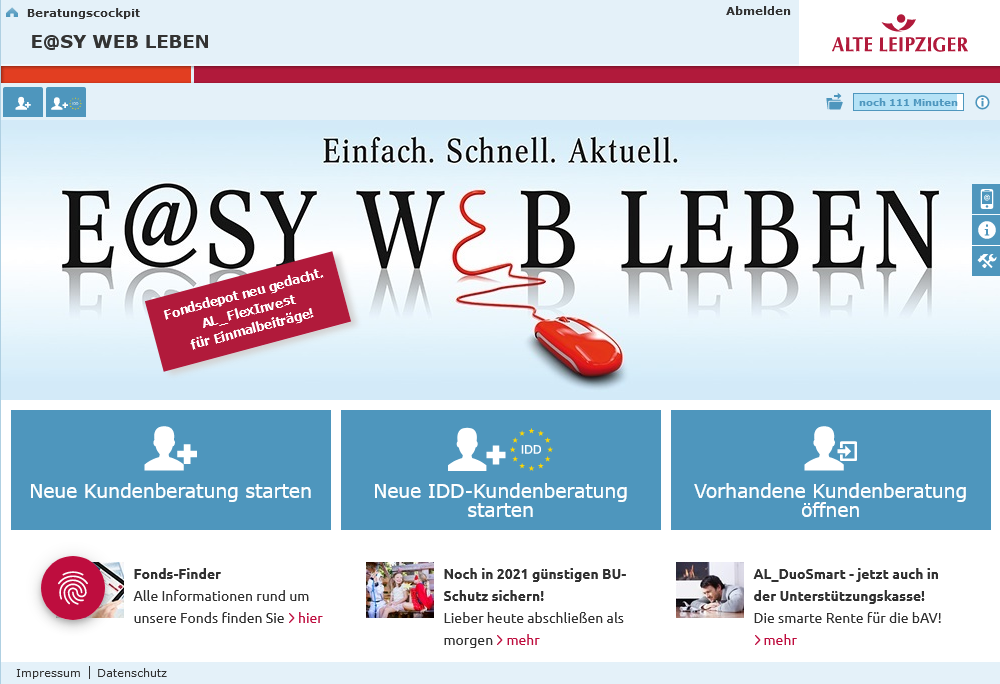
\includegraphics[width=0.8\columnwidth]{images/Easy_Web_Leben_allgemein.png}
\caption{Das Hauptmenü von Easy Web \cite{easy_web}: Es können Kundenprofile zur Kalkulation verschiedener Altersvorsorgeprodukte angelegt und gespeichert werden. Zudem besteht die Möglichkeit ein Kund*innenprofil im Rahmen der IDD-Versicherungsvertriebsrichtlinie anzulegen.}
\label{fig:easyWeballg}
\end{figure}

Verschiedene Konzepte der privaten und betrieblichen Altersvorsorge stehen bei Easy Web zur Auswahl. Mittels einer Registerkarte können Nutzer*innen von Easy Web bei einer Kund*innenberatung zwischen der Bereichen der privaten und betrieblichen Altersvorsorge wechseln. Für beide Bereiche steht zudem eine weitere Registerkarte bereit, die zwischen Rentenprodukten, Berufsunfähigkeitsprodukten und Risikolebensversicherungen unterscheidet. Für jede dieser Registerkarte erscheinen mehrere Tarife, die zur Kalkulation ausgewählt werden können. Der Anwendungsfall dieser Arbeit beschränkt sich auf den Bereich der betrieblichen Altersvorsorge und den Bereich der Renten- beziehungsweise 'Vorsorge'-Produkte. Dies entspricht der Zahlung einer lebenslangen Altersrente, einer einmaligen Rentenauszahlung oder einer Mischung aus den beiden zuvor genannten Varianten bei Erreichen des vordefinierten Rentenalters. Abbildung \ref{fig:easyWebAuswahl} zeigt das Auswahlmenü für den Fall der bAV.

\begin{figure}[t]
\centering
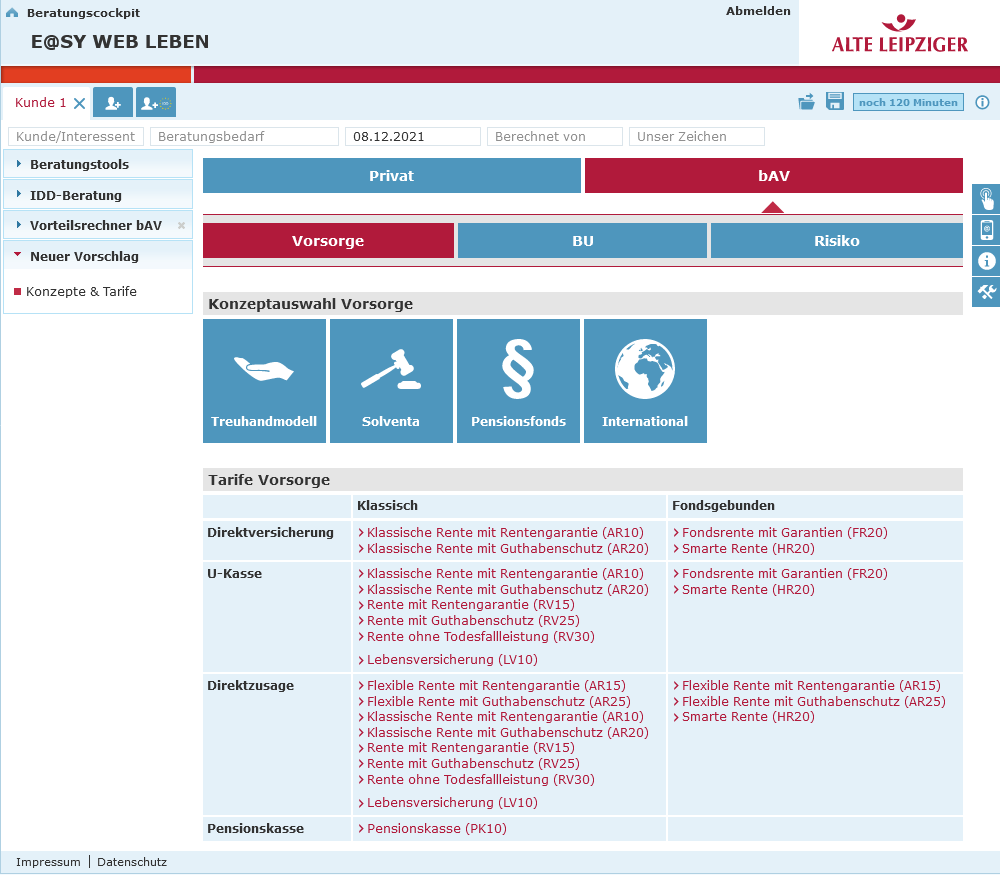
\includegraphics[width=0.7\columnwidth]{images/Easy_Web_Leben_Auswahl.png}
\caption{Das Auswahlmenü von Easy Web bei einer Kund*innenberatung: Es wird zwischen privater und betrieblicher Altersvorsorge unterschieden, zudem können Tarife verschiedener Durchführungswege ausgewählt werden.}
\label{fig:easyWebAuswahl}
\end{figure}

Easy Web ermöglicht die Auswahl von Produkten der bAV über vier der fünf möglichen Durchführungswege (vgl. \autoref{subsec:versicherungsgrundlagen}), die je nach Wahl des Durchführungsweges über eines der verbundenen Unternehmen der ALH-Gruppe abgewickelt werden \cite{alh_bav}:
\begin{itemize}
\item Direktversicherung: Abgewickelt über die Alte Leipziger Lebensversicherung a.G.
\item Unterstützungskasse: Abgewickelt über die Alte Leipziger Unterstützungskasse e.V., rückdeckungsversichert über die Alte Leipziger Lebensversicherung a.G.
\item Direktzusage: Abgewickelt über die Alte Leipziger Lebensversicherung a.G. als Rückdeckungsversicherung für eine Direktzusage eines Unternehmens.
\item Pensionskasse: Abgewickelt über die Alte Leipziger Pensionskasse AG
\end{itemize} 

Zudem unterscheidet Easy Web in klassische und fondsgebundene Tarife. Bei fondsgebundenen Tarifen setzt sich die Anlage des Vertragsguthabens aus dem Deckungskapital der Versicherungsgesellschaft, dem Wertsicherungsfonds und den einem individuell gewählten Fonds zusammen \cite{alh_produkte}. Bei klassischen Tarifen hingegen wird das Guthaben der Kund*innen einzig im Deckungskapital des Versicherers angelegt \cite{alh_produkte}.

Im folgenden werden die verschiedenen Tarife vorgestellt, welche bei Easy Web ausgewählt werden können. Die Erläuterungen basieren auf \cite{alh_produkte}:
\begin{itemize}
\item Rente mit Rentengarantie (RV15) / mit Guthabenschutz (RV25) / ohne Todesfallleistung (RV30): Die Beiträge der Versicherten wandern bei diesen Tarifen vollständig in das Deckungskapital der Alten Leipziger Lebensversicherung a. G. und werden vollständig garantiert. Zusätzlich bestimmt die Wahl des Tarifs zusätzliche Bausteine im Todesfall des Leistungsempfängers: Bei Wahl der Rentengarantie wird ein Zeitraum bestimmt, bis zu welchem die Rente auch an Hinterbliebene weiterhin ausbezahlt wird, bei Wahl des Guthabenschutzes wird das verbleibende Guthaben nach Abzug der bereits gezahlter Renten an Hinterbliebene ausbezahlt. Die dritte Variante verzichtet auf jegliche Leistungen im Todesfall. Diese drei Tarife können bei Easy Web nur über die Durchführungswege der (rückdeckungsversicherten) Direktzusage oder Unterstützungskasse ausgewählt werden.

\item Moderne klassische Rente mit Rentengarantie (AR10) / mit Guthabenschutz (AR20): Die Tarife AR10 und AR20 gleichen in ihrer Anlagestruktur der Tarife RV15, RV25 und RV30. Die Beiträge werden im Deckungsstock in sichere Kapitalanlagen investiert und werden für die Rentenbezugszeit garantiert. Die moderne klassische Rente ermöglicht zudem eine flexible Gestaltung der Beitragshöhe und bietet laut der ALH-Gruppe \cite{alh_produkte} die Chance auf höhere Überschüsse als herkömmliche klassische Renten.
\item Flexible Rente mit Rentengarantie (AR15) / mit Guthabenschutz (AR15): 

\item Fondsrente mit Garantien (FR20): Dieser Tarif gleicht der klassischen Rente mit Rentengarantie (AR10) mit Ausnahme der Anlagestrategie des Vertragsguthabens. Diese geht als Beispiel eines fondsgebundenen Tarifs -- wie zuvor beschrieben -- über das Deckungskapital des Versicherers hinaus und ermöglicht die Wahl eines individuellen Investmentfonds. Die Fondsrente mit Garantien kann via Direktversicherung und Unterstützungskasse durchgeführt werden.
\item Smarte Rente (HR20): Die smarte Rente entspricht ebenfalls einem fondsgebundenen Tarif, der wie auch die Fondsrente mit Garantien neben der klassischen Anlage auf eine dynamische Anlage in einen Investmentfonds setzt. Dieser wird bei der smarten Rente jedoch von der ALH-Gruppe vorgegeben. Zudem unterscheidet sich die smarte Rente gegenüber der Fondsrente derart, dass bei der smarten Rente das Vertragsguthaben vor Rentenbeginn umgeschichtet wird, sodass das garantierte Kapital des Vertrages zu Rentenbeginn sichergestellt ist. Die möglichen Durchführungswege der smarten Rente sind die Direktversicherung, die Unterstützungskasse und die Direktzusage.
\end{itemize}

Wählt man nun einen der zur Verfügung stehenden Tarife aus, öffnet sich eine Eingabemaske zur Eingabe verschiedener Parameter, welche zur Rentenkalkulation zur Rate gezogen werden. Neben Angaben zur versicherten Person müssen Nutzer*innen von Easy Web zudem Informationen zum gewählten Tarif, eventuellen Zusatzversicherungen und der optionalen Beitragsdynamik angeben. Darüber hinaus werden je nach Wahl des Tarifs und Durchführungsweges detaillierte Angaben zum Versicherungsschutz verlangt: Dies umfasst bei allen Tarifen den Versicherungsbeginn, die Art der Finanzierung, die Höhe des Beitrags, das Renteneintrittsalter und die Periodizät der Beitragszahlungen. Ein weiteres Fenster unter der Bezeichnung 'Details', das jedoch nur bei bestimmten Tarifen angezeigt wird, erlaubt zudem die Angabe zusätzlicher detaillierter Faktoren: So können dort beispielsweise Zuzahlungen zu Beginn des Vertragsabschlusses (bei den Durchführungswegen Direktversicherung, Pensionskasse, Direktzusage) oder die genutzten Freibeträge im Sinne von § 3 Nr. 63 EStG und § 40 b EStG (bei den Durchführungswegen Pensionskasse und Direktversicherung, vgl. \autoref{subsec:versicherungsgrundlagen}) spezifiziert werden. Abbildung \ref{fig:easyWebEingabe} zeigt die Eingabemaske beispielhaft für den Tarif 'Klassische Rente mit Rentengarantie (AR10)' des Durchführungswegs Direktversicherung.

\begin{figure}
\centering
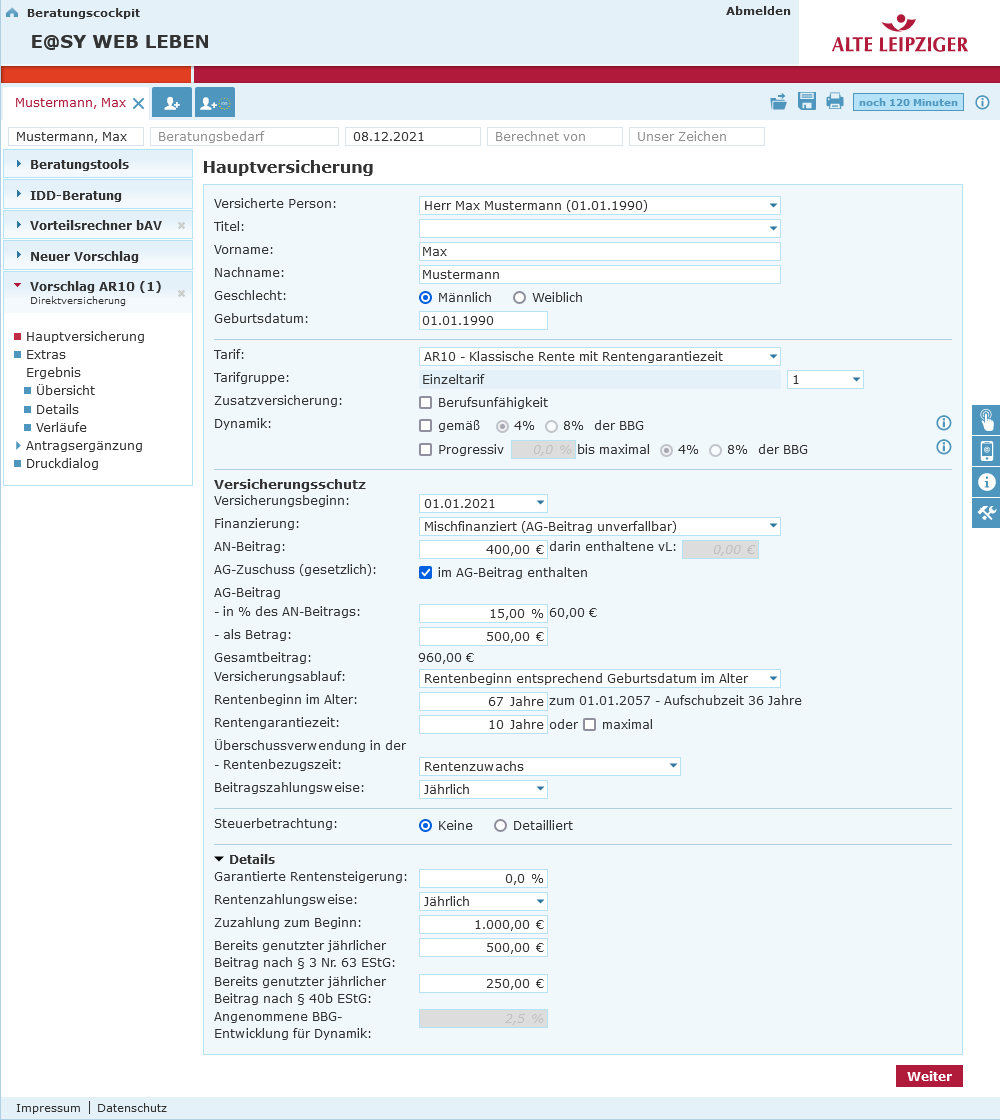
\includegraphics[width=0.9\columnwidth]{images/Easy_Web_Eingabe.png}
\caption{Die Eingabemaske für den Tarif 'Klassische Rente mit Rentengarantie (AR10)' des Durchführungswegs Direktversicherung. Im oberen Bereich werden Angaben zur versicherten Person verlangt, darunter folgt die Spezifizierung der Parameter für den Tarif selbst.}
\label{fig:easyWebEingabe}
\end{figure}

Nach Ausfüllen dieser einführenden Eingabemaske zu Beginn des Kalkulationsprozesses führt Easy Web Nutzer*innen durch weiterführende Formularfelder: Diese können unter anderem die Spezifizierung der Zusatzversicherungen oder die Wahl der Kapitalanlage bei fondsgebundenen Tarifen sein. Anschließend berechnet Easy Web ein Ergebnis für die garantierte und zu erwartendende Rente

\section{Implementierung}



\subsection{Grundlegende Fragestellung}

- Berücksichtigung der vollständigen Kombinatorik für Durchführungsweg und Art der Rueckdeckung

\subsection{Vergleich von Combinatorial Testing Tools/Algorithmen}

\subsection{Combinatorial Testing vs. Random Testing}

\section{Ergebnisse}

\subsection{Grundlegende Fragestellung}

- Berücksichtigung der vollständigen Kombinatorik für Durchführungsweg und Art der Rueckdeckung

\subsection{Vergleich von Combinatorial Testing Tools/Algorithmen}

\subsection{Combinatorial Testing vs. Random Testing}